% This is samplepaper.tex, a sample chapter demonstrating the
% LLNCS macro package for Springer Computer Science proceedings;
% Version 2.20 of 2017/10/04
%

\documentclass[runningheads]{llncs}
%
\usepackage[utf8]{inputenc}
\usepackage[utf8]{vietnam}
\usepackage{graphicx}
\usepackage{epstopdf}
\usepackage{float}
\usepackage{array}
\usepackage{multirow}
\usepackage{ulem}
\usepackage[hyphens]{url}

% Used for displaying a sample figure. If possible, figure files should
% be included in EPS format.
%
% If you use the hyperref package, please uncomment the following line
% to display URLs in blue roman font according to Springer's eBook style:
% \renewcommand\UrlFont{\color{blue}\rmfamily}

\begin{document}
%
\title{Phân tích ảnh hưởng của các chỉ số sức khỏe đến tiến triển bệnh đái tháo đường \thanks{Hướng dẫn bởi TS. Đỗ Trọng Hợp}}
%
%\titlerunning{Abbreviated paper title}
% If the paper title is too long for the running head, you can set
% an abbreviated paper title here
%
\author{Thái Minh Triết\inst{1} \and
Chu Hà Thảo Ngân\inst{2} \and
Võ Tuấn Anh\inst{3} \and
Đỗ Trọng Hợp\inst{4}
}
%
\authorrunning{Thái Minh Triết, Chu Hà Thảo Ngân , Võ Tuấn Anh}
% First names are abbreviated in the running head.
% If there are more than two authors, 'et al.' is used.
%
\institute{Trường Đại học Công nghệ thông tin, Đại học quốc gia Thành phố Hồ Chí Minh \and
Khoa Khoa học và Kỹ thuật Thông tin\\
\email{\{\inst{1}19522397,\inst{2}19521882,\inst{3}19521226\}@gm.uit.edu.vn\\
{\inst{4}hopdt}@uit.edu.vn}}

%
\maketitle              % typeset the header of the contribution
%
\begin{abstract}
Bệnh đái tháo đường theo giới y khoa là một trong những mối đe doạ sức khoẻ toàn cầu đối với cộng đồng có tỉ lệ người mắc ngày càng tăng đều theo từng năm với nhiều nguyên nhân ảnh hưởng, trong đó nguyên nhân chính là rối loạn chức năng chuyển hóa insulin. Nhằm tìm hiểu được các yếu tố bên trong cơ thể có tác động như thế nào đến sự rối loạn này, nhóm chúng tôi đã tìm hiểu các chỉ số y tế mang tính thống kê có liên quan bằng bộ dữ liệu có sẵn và tiến hành phân tích, xử lí và đánh giá để có được những kết quả phù hợp cho mục đích của bài nghiên cứu. Trong quá trình phân tích có sử dụng phương pháp thống kê phân tích hồi quy để tìm ra sự ảnh hưởng và tương tác lẫn nhau của các yếu tố này. Sau khi thực hiện xây dựng các mô hình máy học phù hợp và đánh giá chúng, kết quả thu được là <KẾT QUẢ ĐÁNH GIÁ> cho mô hình phân tích tốt nhất <MÔ HÌNH TỐT NHẤT>. <Lược ý kết luận>

\keywords{Đái tháo đường \and Bệnh tiểu đường \and  Phân tích hồi quy}
\end{abstract}
%
%
%
\section{Giới thiệu chung}

Đái tháo đường được xem là một căn bệnh phổ biến trong cộng đồng, đặc biệt là Mỹ với xu hướng gia tăng ngày càng cao với con số ước tính lên đến 79 triệu người trưởng thành mắc bệnh và trong đó 50\% người mắc đái tháo đường không biết mình có bệnh vì chưa có triệu chứng rõ ràng. 

Đái tháo đường là một căn bệnh liên quan đến sự rối loạn chuyển hóa trong hormone tuyến tuỵ dẫn đến thiếu hụt lượng insuline trong máu. Các tiêu chuẩn để xác định, chuẩn đoán bệnh đái tháo đường hiện nay được Hiệp hội Đái tháo đường Mỹ công bố cần dựa vào nhiều chỉ số và quá trình phức tạp. Ví dụ khi kiểm tra chỉ số HbA1c của bệnh nhân cần được thực hiện ở phòng thí nghiệm được chuẩn hóa cao. Tuy nhiên, cũng nhờ đó mà việc chuẩn đoán đái tháo đường hay tiền đái tháo đường sẽ phần lớn phụ thuộc vào các chỉ số này từ cơ thể. 
Chính vì đó, ta cần phải có được một bộ dữ liệu với các chỉ số y tế liên quan để có thể đánh giá phần nào tình trạng hiện tại của bệnh, giúp tăng hiệu quả cũng như giảm đi chi phí cho quá trình chuẩn đoán. 

Trong bài nghiên cứu này, bộ dữ liệu thu thập được từ các bệnh nhân đái tháo đường với các chỉ số y tế liên quan sẽ được đánh giá bằng các mô hình phân tích hồi quy. Từ đó không chỉ hỗ trợ tích cực cho việc chuẩn đoán mà còn có thể phân tích được sự ảnh hưởng và tương tác giữa các chỉ số trên với nhau.

Cấu trúc bài báo cáo được trình bày như sau: Ở mục 2, chúng tôi trình bày thông tin chi tiết của bộ dữ liệu được sử dụng trong bài nghiên cứu. Ở mục 3, chúng tôi tiếp cận bộ dữ liệu và thực hiện tiền xử lý dữ liệu. Sau khi bộ dữ liệu đã được xử lí, chúng sẽ được đưa vào phân tích bằng các mô hình hồi quy khác nhau, quá trình này sẽ được trình bày ở mục 4. Mục 5 sẽ trình bày kết quả đánh giá các mô hình, từ đó có được mô hình tốt nhất trên bộ dữ liệu. Và cuối cùng ở mục 6 là kết luận và hướng phát triển.

\section{Tổng quan bộ dữ liệu}

\subsection{Giới thiệu chung về bộ dữ liệu}
Bộ dữ liệu được xây dựng bao gồm  thuộc tính cơ bản của 442 bệnh nhân bệnh tiểu đường và kết quả là một giá trị đáng giá quá trình tiến triển của bệnh nhân sau 1 năm ghi nhận. Dưới đây là ví dụ các điểm dữ liệu được trích ra từ bộ dữ liệu và codebook của bộ dữ liệu.
\begin{table}
	\setlength{\tabcolsep}{0.5em}
	\renewcommand{\arraystretch}{1.4}
	\begin{center}
		\caption{Ví dụ về các điểm dữ liệu}\label{tab1}
		\begin{tabular}{|p{0.75cm}|p{0.75cm}|p{0.75cm}|p{0.75cm}|p{0.75cm}|p{0.75cm}|p{0.75cm}|p{0.75cm}|p{1cm}|p{0.75cm}|p{0.75cm}|}
			\hline
			\textbf{AGE}&\textbf{SEX}&\textbf{BMI}&\textbf{BF}&\textbf{S1}&\textbf{S2}&\textbf{S3}&\textbf{S4}&\textbf{S5}&\textbf{S6}&\textbf{Y}\\
			\hline
			59&2&32.1&101&157&93.2&38&4&4.8598&87&151\\
			\hline
			48&1&21.6&87&183&103.2&70&3&3.8918&69&75\\
			\hline
			72&2&30.5&93&156&93.6&41&4&4.6728&85&141\\
			\hline
			24&1&25.3&84&198&131.4&40&5&4.8903&89&206\\
			\hline
			50&	1	&23&	101&	192&	125.4&	52&	4&	4.2905&	80&	135\\
			\hline
		\end{tabular}
	\end{center}
\end{table}

\begin{table}[H]
	\setlength{\tabcolsep}{0.5em}
	\renewcommand{\arraystretch}{1.4}
	\begin{center}
		\caption{Codebook của bộ dữ liệu}\label{tab2}
			\begin{tabular}{ | p{2.5cm} | p{9.45cm} |} 
			\hline
			\textbf{Thông tin} & \textbf{Nội dung}\\ 
			\hline
			Tên bộ dữ liệu &Diabetes dataset\\
			\hline
			Nguồn thu nhập & \url{https://www4.stat.ncsu.edu/~boos/var.select/diabetes.html}\\
			\hline
			Số điểm dữ liệu & 442\\
			\hline
			Số thuộc tính & 11\\
			\hline
			\multirow{1}{2.25cm}
			{Thông tin thuộc tính} & \textbf{AGE:} độ tuổi của bệnh nhân\\
								&\textbf{SEX:} giới tính của bệnh nhân \\
								& -  Giá trị 1 tương ứng với giới tính là Nam\\
								& -  Gái trị 2 tương ứng với giới tính là Nữ\\
								&\textbf{BMI:} Body Mass Index (chỉ số khối cơ thể)\\
								&\textbf{BP:}  average blood pressure (giá trị huyết áp trung bình)\\
								&\textbf{S1:} tổng lượng cholesterol trong huyết thanh (tc - total serum cholesterol)\\
								&\textbf{S2:} giá trị lipoprotein tỷ trọng thấp (ldl - low-density lipoproteins) \\
								&\textbf{S3:} giá trị lipoprotein tỷ trọng cao (hdl - high-density lipoproteins)\\
								&\textbf{S4:} tỉ lệ giữa  cholesterol toàn phần so với lượng HDL (tch - total cholesterol / HDL) \\
								&\textbf{S5:} mức triglyceries có trong huyết thanh có thể ghi nhận (ltg - possibly log of serum triglycerides level)\\
								&\textbf{S6:}  chỉ số mức đường huyết (glu - blood sugar level)\\
								&\textbf{Y:} giá trị định lượng về tiến triển bệnh của bệnh nhân sau 1 năm kể từ thời điểm ghi nhận\\
								\hline
			Tác giả & Bradley Efron, Trevor Hastie, Iain Johnstone và Robert Tibshirani, Đại học Stanford\\
			\hline
			\end{tabular}
		\end{center}
	\end{table}
\subsection{Phân tích và trực quan bộ dữ liệu}

\section{Tiền xử lý dữ liệu}

\subsection{Xử lý ngoại lệ}

\subsection{Chuyển đổi dữ liệu}

\subsection{Phân chia tập train và test}

\section{Phân tích hồi quy}

\subsection{Tổng quan về Phân tích Hồi quy (Regression Analysis)}
Phân tích hồi quy là một phương pháp thống kê mạnh mẽ cho phép xem xét mối tương quan giữa các biến số trong việc đo lường. Có nhiều loại phân tích hồi quy khác nhau nhưng chúng tựu chung đều tập trung vào việc đánh giá sự ảnh hưởng của các biến số độc lập lên một biến phụ thuộc.

Đây cũng là một phương pháp đáng tin cậy để xác định xem liệu biến số nào có ảnh hưởng đến bài toán đo lường (topic of interest). Quá trình thực hiện hồi quy cho phép xác định được yếu tố nào đáng quan tâm nhất và những yếu tố nào có thể bỏ qua, hay sự ảnh hưởng, tương tác lẫn nhau của các yếu tố.

Để hiểu một cách đầy đủ về phương pháp phân tích hồi quy, trước hết cần phải nắm vững một vài thuật ngữ sau:
\begin{itemize}
	\item \textbf{Biến phụ thuộc}: yếu tố chính cần được ước lượng, hiểu rõ và dự đoán 
	\item \textbf{Biến độc lập}: những yếu tố được giả thiết rằng có ảnh hưởng đến biến phụ thuộc
\end{itemize}

\subsection{Phân tích ảnh hưởng của yếu tố}

\subsection{Tương tác giữa các yếu tố}

\subsection{Các độ đo đánh giá mô hình hồi quy}
Đánh giá mô hình là một bước quan trọng không thể thiếu trong quá trình xây dựng mô hình máy học. Đánh giá mô hình hỗ trợ trong việc đánh giá hiệu suất của mô hình trên dữ liệu huấn luyện và phát hiện ra những trường hợp gây ảnh hưởnng tới mô hình như over-fitting (hiện tượng mô hình thể hiện chính xác các điểm dữ liệu huấn luyện) hay under-fitting (hiện tượng mô hình không hoàn toàn có mối liên hệ nào với bộ dữ liệu huấn luyện), từ đó cải thiện chất lượng hiệu suất của mô hình và giúp mô hình đưa ra kết quả khả quan hơn khi xuất hiện bộ dữ liệu mới trong tương lai. Độ đo được sử đụng để đánh giá cho các mô hình máy học hồi quy trong bài báo cáo là Adjusted R-Squared.


\subsubsection{R-Squared}
\begin{equation}
	R-Squared = 1- \frac{SSE}{SST} =  1 - \frac{\sum (Ytrue - Ypred)^2}{\sum (Ytrue - \overline{Y})^2}
\end{equation}
Trong đó:\\
- SSE là Sum of Squared estimate of errors (tổng bình phương lỗi giữa biến phụ thuộc trong bộ dữ liệu với biến phụ thuộc được dự đoán từ mô hình).\\
- SST là sum of squares total (tổng bình phương lỗi giữa giá trị biến phụ thuộc trong bộ dữ liệu với tổng bình phương của nó).\\

Độ đo đánh giá R-Squared hay còn được còn có tên gọi khác là Coefficient of Determination, có khoảng giá trị từ 0 tới 1, giúp nhận xét mức độ thích hợp giữa mô hình và các điểm dữ liệu huấn luyện. Kết quả của độ đo R-Squared không đánh giá hiệu suất của mô hình một cách toàn vẹn, giá trị của độ đo thấp không có nghĩa là mô hình có hiệu suất thấp, ngược lại thì kết quả độ đo có cao thì không đồng nghĩa rằng mô hình hoạt động tốt. Ngoài ra, độ đo R-Squared còn có nhược điểm khi tăng số lượng thuộc tính độc lập thì giá trị của độ đo cũng tăng theo, dẫn tới tăng độ phức tạp cho mô hình mặc dù những thuộc tính mới không hoàn toàn mang ý nghĩa cho việc cải thiện dự đoán biến phụ thuộc.

\subsubsection{Adjusted R-Squared}
\begin{equation}
	Adjusted  R-Squared = 1- (1-R^2)\frac{n-1}{n-p-1}
\end{equation}
Trong đó: \\
- $R^2$: giá trị của R-Square trên bộ dữ liệu.\\
- n: số lượng điểm dữ liệu trong bộ dữ liệu.\\
- p: số lượng thuộc tính độc lập trong bộ dữ liệu.\\

 Độ đo đánh giá Adjusted R-Squared đã khắc phục khuyết điểm vốn có của R-Squared, khi tăng số lượng thuộc tính độc lập nếu giá trị của độ đo Adjusted R-Squared giảm nghĩa là thuộc tính đó không có ý nghĩa trong việc nâng cao hiệu suất mô hình tránh trường hợp dư thừa hay tăng độ phức tạp cho mô hình một cách không cần thiết.


\subsection{Xây dựng mô hình hồi quy}
\subsubsection{Simple Linear Regression}
\subsubsection{Multiple Linear Regression}
\subsubsection{Polynomial Regression}

\subsubsection{Ridge Regression}
là phương pháp xác định hệ số của mô hình hồi quy đa biến trong điều kiện biến độc lập có sự tương quan chặt chẽ với nhau. Được xem là dạng chính quy (regularization) của hồi quy tuyến tính. Dùng để giảm số lượng biến độc lập trong mô hình hồi quy, nhằm giảm các vấn đề Overfitting và Underfitting.
	\begin{equation}
	L_{ridge}(\hat{\beta})=\sum^{n}_{i=1}{(y_i-x'_i\hat{\beta})^2}+\lambda\sum^{m}_{j=1}{\hat{\beta}^2_j}=||y-X\hat{\beta}||^2+\lambda||\hat{\beta}||^2
	\end{equation}

\subsubsection{Lasso Regression}
là một phương phá dùng để giảm số lượng biến độc lập tring mô hình hồi quy nhưng sử dụng tổng các giá trị tuyệt đối của hệ số bên trong biểu thức. Vì về bản chất, Lasso Regression không chỉ giảm giá trị của hệ số mà thậm chí cố gắng loại bỏ nó. Sự khác biệt của Ridge và Lasso là Ridge sẽ không bao giờ cho giá trị của hệ số bằng 0. Hạn chế chính là không phù hợp cho một số loại dữ liệu.
	\begin{equation}
	L_{lasso}(\hat{\beta})=\sum^{n}_{i=1}{(y_i-x'_i\hat{\beta})^2}+\lambda\sum^{m}_{j=1}{|\hat{\beta}_j|}
	\end{equation}

\subsubsection{Elastic Net Regression}
là sự kết hợp của cả hai mô hình Ridge Regression và Lasso Regression. Ưu điểm của mô hình này là không dễ dàng loại bỏ hệ số cộng tuyến.
	\begin{equation}
		L_{enet}(\hat{\beta})=\frac{\sum^{n}_{i=1}{(y_i-x'_i\hat{\beta})^2}}{2n}+\lambda(\frac{1-\alpha}{2}\sum^{m}_{j=1}{\hat{\beta}^2_j+\alpha\sum^{m}_{j=1}{|\hat{\beta}_j|}})
	\end{equation}
\section{Đánh giá mô hình hồi quy}

\subsection{Kết quả đánh giá mô hình}

\subsection{Mô hình tốt nhất}

\section{Kết luận}

\begin{thebibliography}{5}

\end{thebibliography}
\pagebreak
%%%%%%%%%%%%%%%%%%%%%%%%%%%%%%%%%%%%%%%%%%%%%%%%%%%%%%SAMPLE%%%%%%%%%%%%%%%%%%%%%%%%%%%%%%%%%%%%%%%%%%%
\section{First Section}
\subsection{A Subsection Sample}
Please note that the first paragraph of a section or subsection is
not indented. The first paragraph that follows a table, figure,
equation etc. does not need an indent, either.

Subsequent paragraphs, however, are indented.

\subsubsection{Sample Heading (Third Level)} Only two levels of
headings should be numbered. Lower level headings remain unnumbered;
they are formatted as run-in headings.

\paragraph{Sample Heading (Fourth Level)}
The contribution should contain no more than four levels of
headings. Table~\ref{tab3} gives a summary of all heading levels.

\begin{table}
\caption{Table captions should be placed above the
tables.}\label{tab3}
\begin{tabular}{|l|l|l|}
\hline
Heading level &  Example & Font size and style\\
\hline
Title (centered) &  {\Large\bfseries Lecture Notes} & 14 point, bold\\
1st-level heading &  {\large\bfseries 1 Introduction} & 12 point, bold\\
2nd-level heading & {\bfseries 2.1 Printing Area} & 10 point, bold\\
3rd-level heading & {\bfseries Run-in Heading in Bold.} Text follows & 10 point, bold\\
4th-level heading & {\itshape Lowest Level Heading.} Text follows & 10 point, italic\\
\hline
\end{tabular}
\end{table}


\noindent Displayed equations are centered and set on a separate
line.
\begin{equation}
x + y = z
\end{equation}
Please try to avoid rasterized images for line-art diagrams and
schemas. Whenever possible, use vector graphics instead (see
Fig.~\ref{fig1}).

\begin{figure}[h]
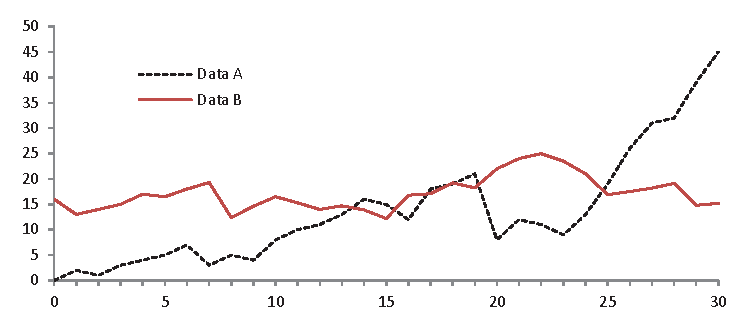
\includegraphics[width=\textwidth]{fig1.eps}
\caption{A figure caption is always placed below the illustration.
Please note that short captions are centered, while long ones are
justified by the macro package automatically.} \label{fig1}
\end{figure}

\begin{theorem}
This is a sample theorem. The run-in heading is set in bold, while
the following text appears in italics. Definitions, lemmas,
propositions, and corollaries are styled the same way.
\end{theorem}
%
% the environments 'definition', 'lemma', 'proposition', 'corollary',
% 'remark', and 'example' are defined in the LLNCS documentclass as well.
%
\begin{proof}
Proofs, examples, and remarks have the initial word in italics,
while the following text appears in normal font.
\end{proof}
For citations of references, we prefer the use of square brackets
and consecutive numbers. Citations using labels or the author/year
convention are also acceptable. The following bibliography provides
a sample reference list with entries for journal
articles~\cite{ref_article1}, an LNCS chapter~\cite{ref_lncs1}, a
book~\cite{ref_book1}, proceedings without editors~\cite{ref_proc1},
and a homepage~\cite{ref_url1}. Multiple citations are grouped
\cite{ref_article1,ref_lncs1,ref_book1},
\cite{ref_article1,ref_book1,ref_proc1,ref_url1}.
%
% ---- Bibliography ----
%
% BibTeX users should specify bibliography style 'splncs04'.
% References will then be sorted and formatted in the correct style.
%
% \bibliographystyle{splncs04}
% \bibliography{mybibliography}
%
\begin{thebibliography}{8}
\bibitem{ref_article1}
Author, F.: Article title. Journal \textbf{2}(5), 99--110 (2016)

\bibitem{ref_lncs1}
Author, F., Author, S.: Title of a proceedings paper. In: Editor,
F., Editor, S. (eds.) CONFERENCE 2016, LNCS, vol. 9999, pp. 1--13.
Springer, Heidelberg (2016). \doi{10.10007/1234567890}

\bibitem{ref_book1}
Author, F., Author, S., Author, T.: Book title. 2nd edn. Publisher,
Location (1999)

\bibitem{ref_proc1}
Author, A.-B.: Contribution title. In: 9th International Proceedings
on Proceedings, pp. 1--2. Publisher, Location (2010)

\bibitem{ref_url1}
LNCS Homepage, \url{http://www.springer.com/lncs}. Last accessed 4
Oct 2017
\end{thebibliography}
\end{document}
